
\section{TraceLogVisualizerの全体像}

TLVの主機能は,2つの主たるプロセスと6種の外部ファイルによって実現される.
図\ref{fig:tlv}にTLVの全体像を示す.

2つの主たるプロセスとは,標準形式への変換と,図形データの生成である.
標準形式への変換は,任意の形式をもつトレースログを標準形式トレースログに変換する処理である.
この処理には,外部ファイルとして変換元のトレースログファイル,リソースを定義したリソースファイル,リソースタイプを定義したリソースヘッダファイル,標準形式トレースログへの変換ルールを定義した変換ルールファイルが読み込まれる.

また,図形データの生成は,変換した標準形式トレースログに対して可視化ルールを適用し図形データを生成する処理である.
この処理には外部ファイルとして可視化ルールファイルが読み込まれる.
可視化ルールファイルとは図形と可視化ルールの定義を記述したファイルである.

TLVは,トレースログとリソースファイルを読み込み,トレースログの対象に対応したリソースヘッダファイル,変換ルールファイルの定義に従い,標準形式トレースログを生成する.
生成された標準形式トレースログに可視化ルールファイルで定義される可視化ルールを適用し図形データを生成した後,画面に表示する.

生成された標準形式トレースログと図形データは,TLVデータとしてまとめられ可視化表示の元データとして用いられる.
TLVデータはTLVファイルとして外部ファイルに保存することが可能であり,TLVファイルを読み込むことで,標準形式変換と図形データ生成の処理を行わなくても可視化表示できるようになる.

図\ref{fig:TLVscreenshot}に,TLVのスクリーンショットを示す.

\begin{figure}[!t]
\begin{center}
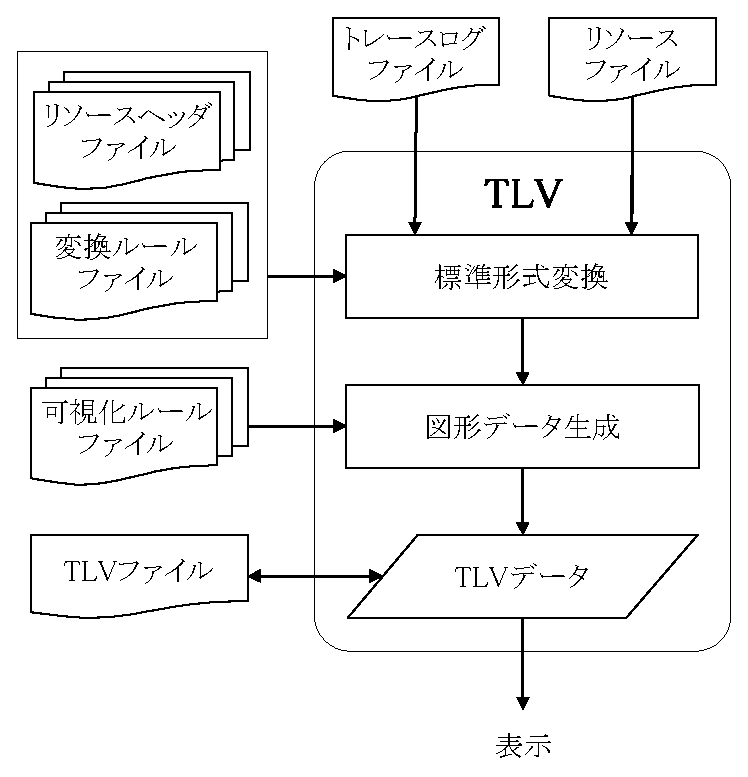
\includegraphics[scale=0.7]{img/tlv.eps}
\caption{TLVの全体像}
\label{fig:tlv}
\end{center}
\end{figure}

\begin{figure}[!t]
\begin{center}
\includegraphics[scale=0.7]{img/TLVscreenshot.eps}
\caption{TLVのスクリーンショット}
\label{fig:TLVscreenshot}
\end{center}
\end{figure}

\subsection{JSON}

リソースファイル,リソースヘッダファイル,変換ルールファイル,可視化ルールファイルは,JSON(JavaScript Object Notation)\cite{JSON}と呼ばれるデータ記述言語を用いて記述する.

JSONは,主にウェブブラウザなどで使用されるECMA-262,revision 3準拠のJavaScript(ECMAScript)と呼ばれるスクリプト言語のオブジェクト表記法をベースとしており,RFC 4627としてで仕様が規定されている.
JSONはUnicodeのテキストデータで構成され,バイナリデータを扱うことはできない.
また,JSONではシンタックスのみの規定がなされ,セマンティクスは規定されていない.

JSONの特徴は,シンタックスが単純であることである.
これは,人間にとっても読み書きし易く,コンピュータにとっても解析し易いことを意味する.
また,複数のプログラミング言語でJSONファイルを扱うライブラリが実装されており,異なる言語間のデータ受け渡しに最適である.
JSONが利用可能なプログラミング言語としては,ActionScript, C, C++, C\#, ColdFusion, Common Lisp, Curl, D言語, Delphi, E, Erlang, Haskell, Java, JavaScript (ECMAScript), Lisp, Lua, ML, Objective CAML, Perl, PHP, Python, Rebol, Ruby, Scala, Squeakなどがある.

TLVの各ファイルのフォーマットにJSONを採用した理由はこれらの特徴による.
シンタックスが単純であることにより,ユーザの記述コスト,習得コストを低減させることができ,また,複数のプログラミング言語でパース可能であることによりファイルに可搬性を持たせることができるからである.

JSONで表現するデータ型は以下のとおりであり,これらを組み合わせることでデータを記述する.
\begin{itemize}
\setlength{\itemsep}{0.5\itemsep}
\item 数値(整数,浮動小数点)
\item 文字列(Unicode)
\item 真偽値(true,false)
\item 配列(順序付きリスト)
\item オブジェクト(ディクショナリ,ハッシュテーブル)
\item null
\end{itemize}

JSONの文法をEBNFと正規表現を用いて説明する.

JSONは,次に示すようにオブジェクトか配列で構成される.

\begin{EBNF}
JSONText = Object | Array;
\end{EBNF}

オブジェクトは複数のメンバをカンマで区切り,中括弧で囲んで表現する.
メンバは名前と値で構成され,名前のあとにはセミコロンが付く.
メンバの名前は値であり,データ型は文字列である.
オブジェクトの定義を次に示す.

\begin{EBNF}
Object = "{",Member,[{",",Member}],"}";
Member = String,":",Value;
\end{EBNF}

配列は複数の値を持つ順序付きリストであり,値をコンマで区切り,角括弧で囲んで表現する.
次に配列の定義を示す.

\begin{EBNF}
Array = "[",Value,[{",",Value}],"]";
\end{EBNF}

値は,文字列,数値,オブジェクト,配列,真偽値,nullのいずれかである.
文字列はダブルクオーテーションで囲まれたUnicode列である.
数値は10進法表記であり,指数表記も可能である.
値の定義を次に示す.

\begin{EBNF}
Value = String|Number|Object|Array|Boolean|"null";
String = /"([^"\]|\n|\"|\\|\b|\f|\r|\t|\u[0-9a-fA-F]{4})*"/;
Boolean = "true"|"false";
Number = ["-"],("0"|Digit1-9,[Digit]),[".",Digit],Exp;
Exp = ["e",[("+"|"-")],Digit];
Digit = /[0-9]+/;
Digit1-9 = /[1-9]/;
\end{EBNF}

表\ref{JSONObject}にJSONにおけるオブジェクトを定義した例を示す.

\begin{FileToPage}{JSONにおけるオブジェクトを定義した例}{JSONObject}
{
  "Image":{
    "Width":  800,
    "Height": 600,
    "Title":  "View from 15th Floor",
    "Thumbnail":{
      "Url":    "http://www.example.com/image/481989943",
      "Height": 125,
      "Width":  "100"
    },
    "IDs": [116, 943, 234, 38793]
  }
}
\end{FileToPage}

表\ref{JSONArray}にJSONにおける配列を定義した例を示す.

\begin{FileToPage}{JSONにおける配列を定義した例}{JSONArray}
[
  {
    "City":      "SAN FRANCISCO",
    "State":     "CA",
    "Zip":       "94107",
    "Country":   "US"
  },
  {
    "City":      "SUNNYVALE",
    "State":     "CA",
    "Zip":       "94085",
    "Country":   "US"
  },
  {
    "City":      "HEMET",
    "State":     "CA",
    "Zip":       "92544",
    "Country":   "US"
  }
]
\end{FileToPage}
